%%
%% labs/common/storylines.tex
%% (c) 2020-22 Christopher A. Bohn
%%
%% Licensed under the Apache License, Version 2.0 (the "License");
%% you may not use this file except in compliance with the License.
%% You may obtain a copy of the License at
%%     http://www.apache.org/licenses/LICENSE-2.0
%% Unless required by applicable law or agreed to in writing, software
%% distributed under the License is distributed on an "AS IS" BASIS,
%% WITHOUT WARRANTIES OR CONDITIONS OF ANY KIND, either express or implied.
%% See the License for the specific language governing permissions and
%% limitations under the License.
%%

\newcommand{\MeetArchie}{
    \begin{wrapfigure}{r}{0.33\textwidth}
        \centering
        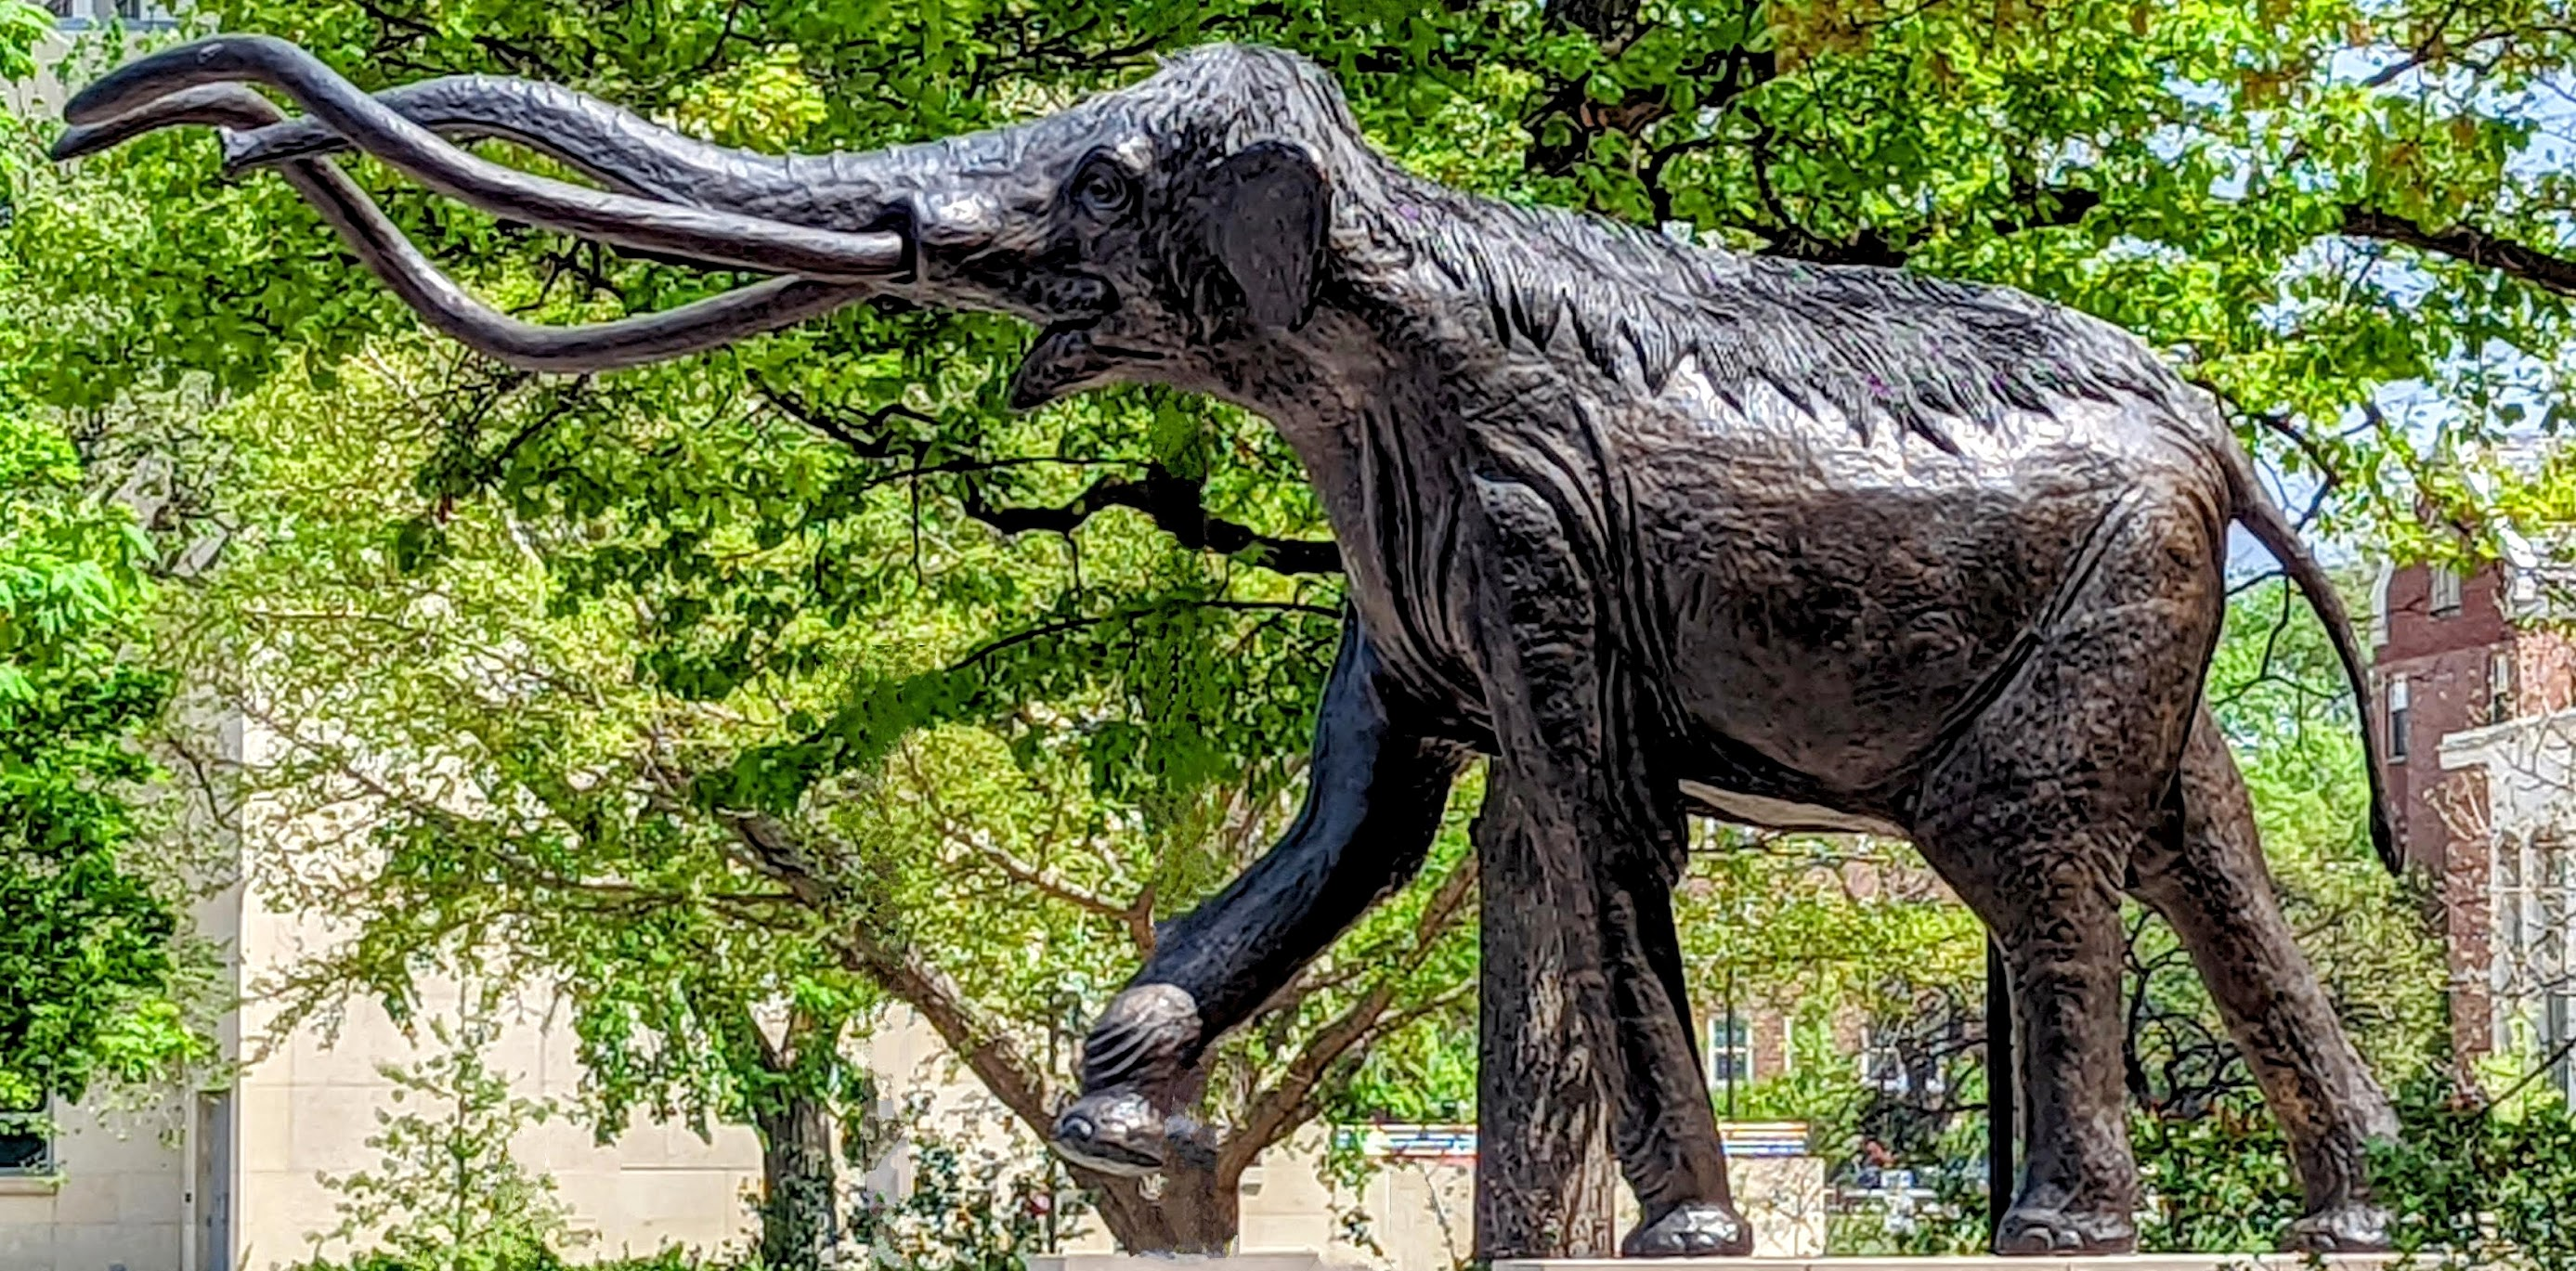
\includegraphics[width=.4\textwidth]{archie}
        \caption{Archie.\\ \footnotesize{Photograph by Bohn.}}
    \end{wrapfigure}

    You're relaxing at your favorite hangout when another customer catches your attention.
    He's rather large (dare I say, \textit{mammoth}), a bit hairy, and looking frustrated in front of his laptop.
    ``I'm Archie,'' he says, ``and I'm trying to teach myself this card game called \textit{Poker}.
    I found this source code that I thought I could use to understand Poker better, but the code is incomplete, and I don't entirely understand what's there.
    Could you explain the code to me, please?'
}

\newcommand{\GetHired}{
    Archie's face lights up in a very big smile.
    ``Thanks!''
    After pausing in thought for a moment, he says, ``Say, I've got a new startup company that could really use your help.
    Are you interested?
    It'll be exciting!''
}

\newcommand{\FirstDayOnTheJob}{
    \begin{wrapfigure}{r}{0.33\textwidth}
        \centering
        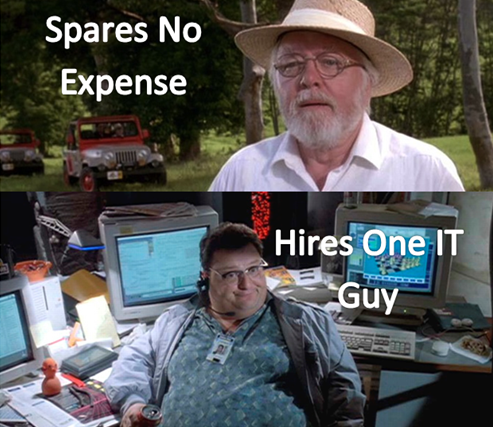
\includegraphics[width=.4\textwidth]{some-expenses-spared}
        \caption{Some expenses were spared.\\ \footnotesize{Original images \textcopyright\ Universal Studios and Amblin Entertainment, Inc. Meme creator unknown.}}
    \end{wrapfigure}

    You've recently been hired to help get the Pleistocene Petting Zoo get started.
    Your new employer, Archie, is surprisingly honest: he admits to you that some expenses were spared.
    Archie cheerfully points out that any challenge is also an opportunity to succeed.
    You suspect your job will offer plenty of ``opportunities to succeed.''
}

\newcommand{\HasKeyboard}{
    Great news!
    Archie brings you your new keyboard.
    He also brings you a problem of his own.
    Because you were held up with the broken keyboard, Archie decided to try some programming on his own, and his code is behaving strangely.
}

\newcommand{\ArchieWroteSmellyCode}{
    Working at the Pleistocene Petting Zoo certainly is proving to be interesting.
    You're glad that you don't have to worry about the problem of the giant sloths very slowly chasing their handlers, but now it seems that Archie has decided to try to write a program or two.
    At a glance, his code is smellier than the wooly rhinoceros' enclosure.
    But you take a closer look anyway to try to understand why his code acts strangely.
}

\newcommand{\InsurancePreview}{
    You hear somebody enter the room.
    ``\textit{Frankenstein}, `boat','' is the challenge, and she answers, ``borne.''
    Archie introduces you to the new arrival, ``Lil, this is our new developer, the one who wrote the app we just used.''
    He turns to you: ``This is Lilith Redd from business operations.''
    He turns back to her and continues, ``Lil, what's the good word?''

    ``The word isn't good, I'm afraid.
    I just heard back from the insurance company.''
}

\newcommand{\OnLoanToEclecticElectronics}{
    All work at the Pleistocene Petting Zoo has stopped while Archie tries to find
    a $\cancelto{\mathrm{reasonable}}{\mathrm{gullible}}$ insurance company. Rather
    than furloughing staff, he's asked everybody to help out with his other startup
    companies for a week or two. He specifically asked that you help out with
    Eclectic Electronics.

    Herb Bee, the chief engineer, explains that Eclectic Electronics is developing
    a patent-pending C-licon tool that will convert C code into an integrated
    circuit that has the same functionality as the original C code. To test it out,
    he tasked you with writing the code to implement an Arithmetic Logic Unit
    (ALU). Your task will be to implement integer addition, subtraction,
    multiplication, and division. Because bitwise operations and bit shift
    operations have been implemented, you will be able to use C's bitwise and bit
    shift operators, but because arithmetic operations have not yet been
    implemented, you cannot use C's arithmetic operators. Because C library
    functions generally make use of arithmetic operations (which have not yet been
    implemented), you cannot use library functions.
}

\newcommand{\SuccessfulALU}{
    Herb smiles as he hands you the the test results from the latest integrated
    circuit fab batch. ``C-licon successfully turned your code into an ALU. Nicely
    done!'' I think maybe it's time to use it to see if we can improve the Floating
    Point Unit (FPU) on our experimental microprocessor.
}

\newcommand{\WriteAnFPU}{
    Herb tells you that, Eclectic Electronics tested the integrated circuit that the C-licon tool created from your ALU code, and they've concluded that C-licon is ready to use for their new experimental microprocessor.
    He tasks you with writing C code (that will be used by the C-licon tool) to implement a Floating Point Unit (FPU).
    Your task will be to implement floating point addition, subtraction, multiplication, and division.
    You can use any bit operations and, thanks to the ALU you wrote, you can use any integer arithmetic operations (use the conventional + - * / operators).
    Because the FPU has not yet been implemented, you cannot use C's floating point operations, you cannot use \lstinline{float}s nor \lstinline{double}s, and you cannot use library functions.
}

\newcommand{\GoingBackToTheZoo}{
    Lil enters the room.
    Herb challenges her: ``\textit{Gulliver's Travels}, `endian','' and Lil answers, ``ends.''

    Lil walks up to you and says, ``We have the insurance situation taken care of, and it's time to get the Zoo ready for guests.
    We're reassembling the tech team, and there's plenty of work to do.''

    You smile.
    ``That's good news!''

    Lil's face is hard to read.
    ``Well, yes and no.
    It's good that you'll be able to resume work on the Zoo's systems.
    But while Archie was waiting for us to fix the insurance situation, he got bored and -- cutting a long story short -- he ended up creating some new `opportunities' that we need you `to succeed' at.''
}

\newcommand{\SettledIntoRoutine}{
    You've settled into a comfortable routine at the Pleistocene Petting Zoo. While
    your job isn't quite as exciting as that of the saber-toothed tigers' dentist,
    it still has something new and interesting almost every day.

    Archie announces that he heard that hand-crafted assembly code can be faster
    than high-level language code. You try to explain that while this may have been
    true decades ago, modern optimizing compilers generate code faster than what a
    typical programmer can achieve with assembly code. Archie doesn't believe you
    and insists that you write the zoo's new cipher program in x86 assembly code.
}

\newcommand{\NewmanRanOffWithSamples}{
    Archie is hurriedly packing is trunk, like he's about to leave on a
    short-notice urgent trip. Before charging out the door, he pauses to tell you,
    ``Newman just stole some of our samples. I need to track him down before he
    sells them to the Supersized Safari Syndicate. I guess this means you're in
    charge of the Zoo's computer system now. Don't worry, you'll be fine. What
    could possibly go wrong?''
}

\newcommand{\BombLabIntroduction}{  % Ties Bryant & O'Halloran's Bomb Lab into the Pleistocene Petting Zoo story
    In a jarring collision of movie franchises, the CEO of Virtucon makes a Zoom
    call to the Pleistocene Petting Zoo. For some reason that nobody really
    explains, you're the only person available to handle the situation. The guy,
    who sounds kind of like an animated ogre, demands that the Pleistocene Petting
    Zoo deliver to him a megalodon shark with a head-mounted laser capable of
    emitting a beam of pure antimatter.

    You blurt out, ``Then it's not a laser,'' and then try to explain to him that
    megalodons are from the Miocene epoch, and expecting to find them at the
    Pleistocene Petting Zoo would be as ridiculous as a Cretaceous-period
    tyrannosaur at a Jurassic-themed park.

    ``Zip it!'' commands the guy who kind of looks like the host of a public-access
    show you used to watch. ``Since you won't meet my demand, my minions have
    placed a `binary bomb' under your zoo. Because I like really convoluted plans,
    we put software on your Linux server that controls the bomb. If you do nothing,
    the bomb will explode. If you turn off the Linux server, the bomb will explode.
    If you go slower than 50mph, the bomb will -- no, never mind that last part.

    ``The bomb software consists of a sequence of phases. Each phase expects you to
    type a particular string on \texttt{stdin}.  If you type the correct string,
    then the phase is {\em defused} and the bomb proceeds to the next phase.
    Otherwise, the bomb {\em explodes}. The bomb is defused when every phase has
    been defused.

    ``Your mission, which you have no choice but to accept, is to defuse your bomb
    before the due date.  Good luck, and welcome to the bomb squad!''
}

\newcommand{\FoodLockersAreStuck}{
    Having saved the Zoo from Dr. Evil's binary bomb, you relax back in your chair and think about taking a break.
%SPRINGBREAK
%   Maybe an entire week in which you don't have solve any problems or meet any deadlines -- that'd be real nice.
%FALLBREAK
    Maybe 4-day weekend in which you don't have solve any problems or meet any deadlines -- that'd be real nice.

    Another Zoom call comes in. \textit{What now!?} you wonder as you take your
    feet off of the desk to answer the call.  An uncomfortable-looking animal
    handler says, ``We can't unlock the food lockers. It's the animals' feeding
    time, and we can't open the food lockers! It's feeding time, we can't get to
    the animals' food, and,'' his eyes dart nervously toward the animal enclosures,
    ``and many of them have sharp, pointy claws and others have big, stompy feet.''
}

\newcommand{\AttackLabIntroduction}{    % Ties Bryant & O'Halloran's Attack Lab into the Pleistocene Petting Zoo story
    You managed to keep the Pleistocene Petting Zoo from blowing to smithereens,
    but it turns out that Dr. Evil's minions weren't too careful when they put the
    bomb control software on the Zoo's Linux server. The software that controls the
    food locker has been heavily damaged! The functions that unlock the food locker
    doors are still present, but there's no way to activate those functions.

    You then recall what Archie told you when he hired you: some expenses were
    spared. You run the machine code through a disassembler and quickly see that it
    has a buffer overflow vulnerability. Before the situation in the dire wolf
    enclosure gets too dire, you sit down and get to work.

    The \function{ctarget} code runs on an older machine that allows executable
    code to be present on the stack, so it's vulnerable to a conventional code
    injection buffer overflow attack.
    \begin{itemize}
        \item Phase 1 (\function{touch1}) unlocks the food locker so the animal handlers can prepare the food.
        \item Phase 2 (\function{touch2}) opens the doors between the food locker and the carnivore enclosures;
        you will need to pass a cookie to the function to authenticate yourself.
        \item Phase 3 (\function{touch3}) closes the doors between the food locker and the carnivore enclosures.
    \end{itemize}
    The \function{rtarget} code runs on a newer machine that does not allow executable code to be present on the stack, so you'll have to conduct a return-oriented programming attack on it.
    \begin{itemize}
        \item Phase 4 (\function{touch2)} opens the doors between the food locker and the herbivore enclosures;
        you will need to pass a cookie to the function to authenticate yourself.
        \item Phase 5 (\function{touch3}) closes the doors between the food locker and the herbivore enclosures.
    \end{itemize}
}

\newcommand{\MostAnimalsAreFed}{
    Before you take on the Phase 5, pause to consider what you have
    accomplished so far.
    In Phases 2 and 3,
    you caused a program to execute machine code of your
    own design.  If {\sc ctarget} had been a network server, you could
    have injected your own code into a distant machine.  In Phase 4, you
    circumvented two of the main devices modern systems use to thwart
    buffer overflow attacks.  Although you did not inject your own code,
    you were able inject a type of program that operates by stitching
    together sequences of existing code.
    Also, all animals have been fed, the carnivores are still in their enclosure, the mammoths can't fit through the herbivore door, and only the giant sloths seem interested in very slowly escaping.
}

\newcommand{\ArchieReturns}{
    Archie returns from tracking down Newman, who'd run off with some of the
    Pleistocene Petting Zoo's samples shortly before Dr.~Evil's Zoom call. ``It
    turns out he didn't get very far at all,'' Archie sighs. ``He ran into a flock
    of terror birds as he was leaving, and we found him in one of the emergency
    shelters.

    Archie smiles. ``I trust things were uneventful while I was away?''
}

\newcommand{\PickingUpNewmansProject}{
    Archie seems genuinely surprised that Newman is refusing to go back to work.
    ``You would think that he'd be grateful for being rescued from that flock of terror birds.''
    Before you can wonder out-loud whether it would be a good idea to trust someone who had just tried to sell trade secrets to a competitor, Archie gives you your new task.

    ``Because Newman isn't cooperating, I need you to finish the project he was working on.
    As you can imagine, duplicating the genetic information for our exhibits can take a long time, and Newman realized that we might be able to duplicate the data faster if we had a concurrent program which has one thread reading from the original data and another thread writing the copy.
    Unfortunately, he ran off to sell samples to the  Supersized Safari Syndicate before finishing the duplicator.
    Right now the duplicator seems to work, but it usually makes imperfect copies.
    Have you ever seen a paleolama with two noses, four eyes, and no ears!?''
}

\newcommand{\WeNeedBetterSecurity}{
    Between Newman trying to samples to a competitor, that weird guy almost blowing up the zoo, and the animals almost escaping, Archie is getting worried.
    ``I think we need to introduce additional protective measures.
    As useful as your challenge-response app is in helping us detect intruders, I think it's now clear that we need something that will detect someone -- or some\textit{thing} -- when they're someplace they shouldn't be, even when no one else is around.
    I've asked the team at Eclectic Electronics to put something together.''
}